\documentclass[11pt,a4paper]{beamer}
\usepackage[ngerman]{babel}
\usepackage[T1]{fontenc}
\usepackage[utf8]{inputenc}
\usepackage{amsmath}
\usepackage{amsfonts}
\usepackage{amssymb}
\usepackage[normalem]{ulem}

\usetheme{Berlin}
\author{Xenia Kühling}
\begin{document}


\begin{frame}{Problemstellung}
\begin{itemize}
\item Koreferenzresolution in BART mit neuem Ansatz: 
\begin{itemize}
\item Vorwiegend regelbasiertes System der Stanford-NLP-Gruppe
\item Bestes Ergebnis bei CoNLL-2011 shared task
\item Adaptiert für Chinesisch, Arabisch
\end{itemize}
\end{itemize}
\end{frame}

\begin{frame}{Input + Mention Detection}
Beispielsatz:
\begin{quote}
John is a musician. He played a new song. A girl was listening to the song. “It is my favorite,” John said to her.
\end{quote} 
\bigskip

[John]$^{1}_{1}$ is [a musician]$^{2}_{2}$. [He]$^{3}_{3}$ played [a new song]$^{4}_{4}$.

[A girl]$^{5}_{5}$ was listening to [the song]$^{6}_{6}$.

“[It]$^{7}_{7}$ is [[my]$^{9}_{9}$ favorite]$^{8}_{8}$,” [John]$^{10}_{10}$ said to [her]$^{11}_{11}$.

\end{frame}

\begin{frame}{Speaker Identification}

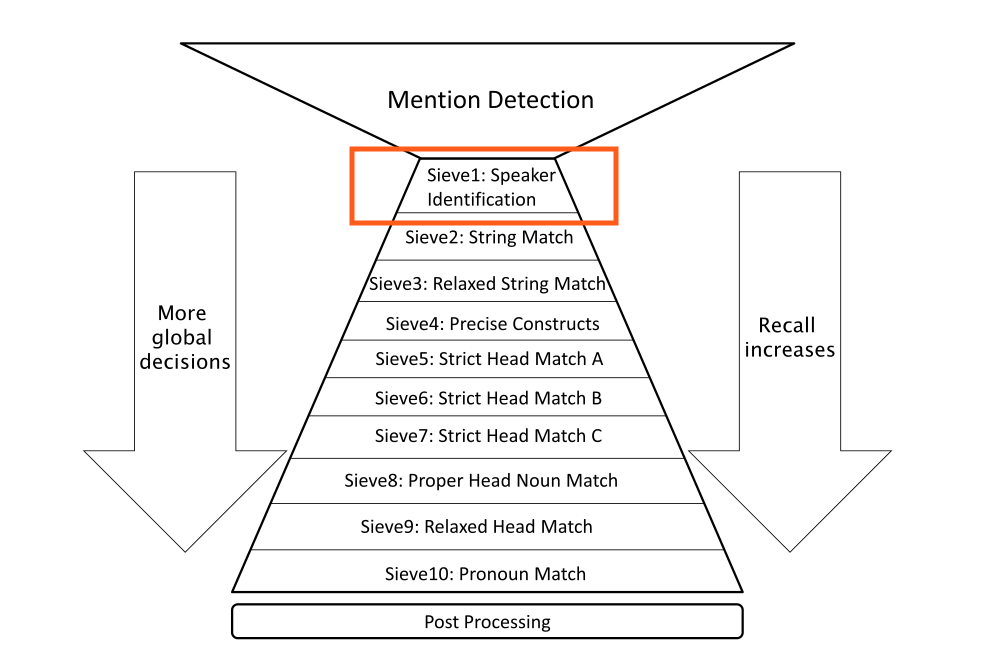
\includegraphics[scale=0.15]{sieve1.png} 
\bigskip

[John]$^{1}_{1}$ is [a musician]$^{2}_{2}$. [He]$^{3}_{3}$ played [a new song]$^{4}_{4}$.

[A girl]$^{5}_{5}$ was listening to [the song]$^{6}_{6}$.

“[It]$^{7}_{7}$ is [\textbf{[my]}$^{9}_{9}$ favorite]$^{8}_{8}$,” \textbf{[John]$^{9}_{10}$} said to [her]$^{11}_{11}$.

\end{frame}

\begin{frame}{String Match}

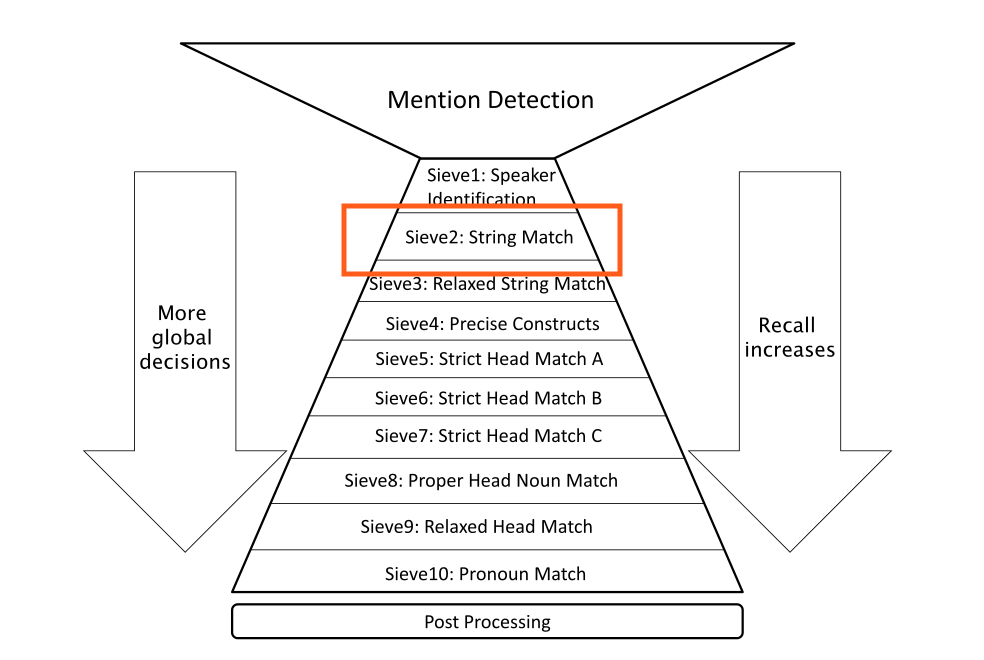
\includegraphics[scale=0.15]{sieve2.png} 
\bigskip

\textbf{[John]$^{1}_{1}$} is [a musician]$^{2}_{2}$. [He]$^{3}_{3}$ played [a new song]$^{4}_{4}$.

[A girl]$^{5}_{5}$ was listening to [the song]$^{6}_{6}$.

“[It]$^{7}_{7}$ is [[my]$^{1}_{9}$ favorite]$^{8}_{8}$,” \textbf{[John]$^{1}_{10}$} said to [her]$^{11}_{11}$.

\end{frame}

\begin{frame}{Relaxed String Match}

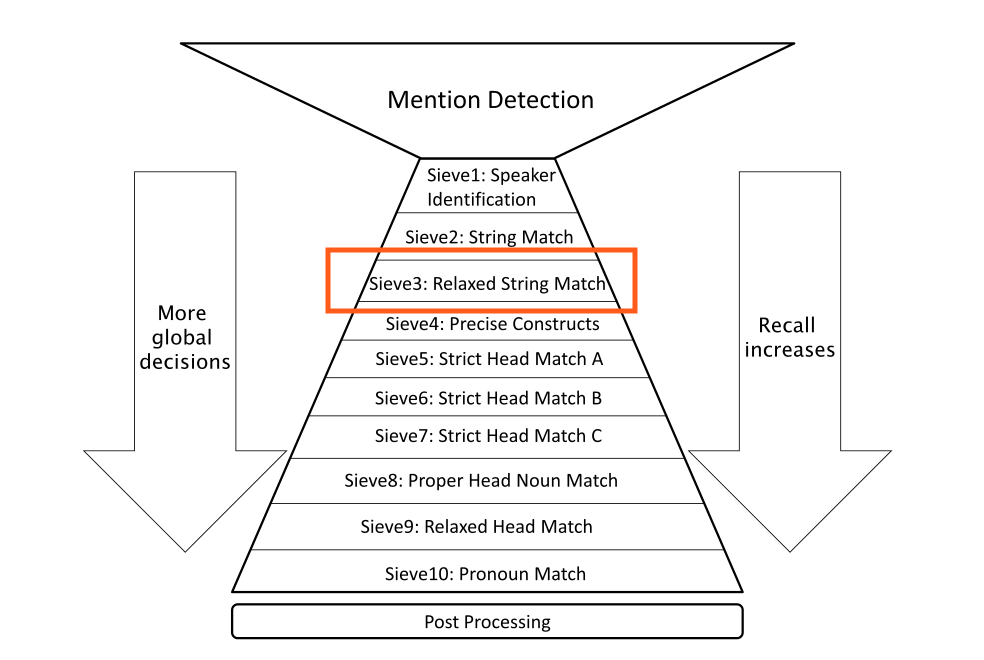
\includegraphics[scale=0.15]{sieve3.png} 
\bigskip

[John]$^{1}_{1}$ is [a musician]$^{2}_{2}$. [He]$^{3}_{3}$ played [a new song]$^{4}_{4}$.

[A girl]$^{5}_{5}$ was listening to [the song]$^{6}_{6}$.

“[It]$^{7}_{7}$ is [[my]$^{1}_{9}$ favorite]$^{8}_{8}$,” [John]$^{1}_{10}$ said to [her]$^{11}_{11}$.

\end{frame}

\begin{frame}{Precise Constructs}

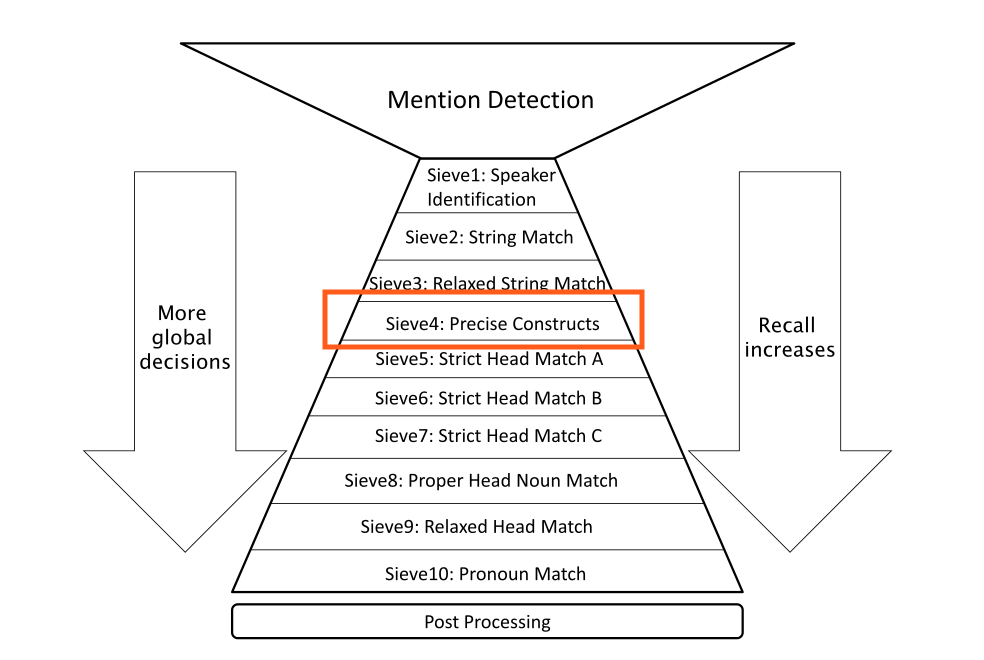
\includegraphics[scale=0.15]{sieve4.png} 
\bigskip

\textbf{[John]}$^{1}_{1}$ is \textbf{[a musician]}$^{1}_{2}$. [He]$^{3}_{3}$ played [a new song]$^{4}_{4}$.

[A girl]$^{5}_{5}$ was listening to [the song]$^{6}_{6}$.

“\textbf{[It]}$^{7}_{7}$ is [\textbf{[my]}$^{1}_{9}$ \textbf{favorite]}$^{7}_{8}$,” [John]$^{1}_{10}$ said to [her]$^{11}_{11}$.

\end{frame}

\begin{frame}{Strict Head Match A}

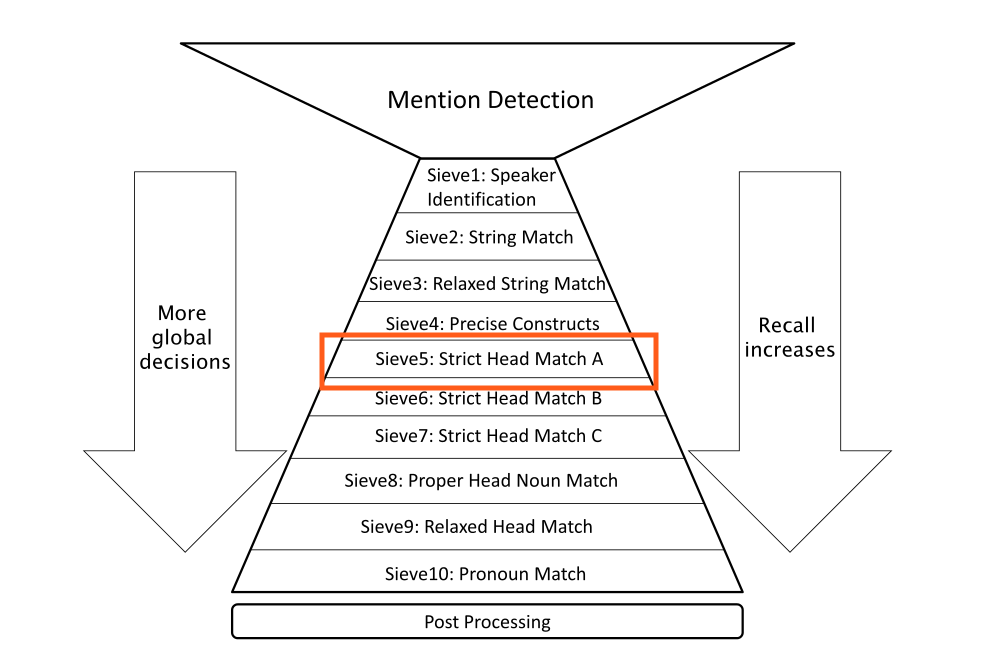
\includegraphics[scale=0.15]{sieve5.png} 
\bigskip

[John]$^{1}_{1}$ is [a musician]$^{1}_{2}$. [He]$^{3}_{3}$ played \textbf{[a new song]}$^{4}_{4}$.

[A girl]$^{5}_{5}$ was listening to \textbf{[the song]}$^{4}_{6}$.

“[It]$^{7}_{7}$ is [[my]$^{1}_{9}$ favorite]$^{7}_{8}$,” [John]$^{1}_{10}$ said to [her]$^{11}_{11}$.

\end{frame}

\begin{frame}{Strict Head Match B C}

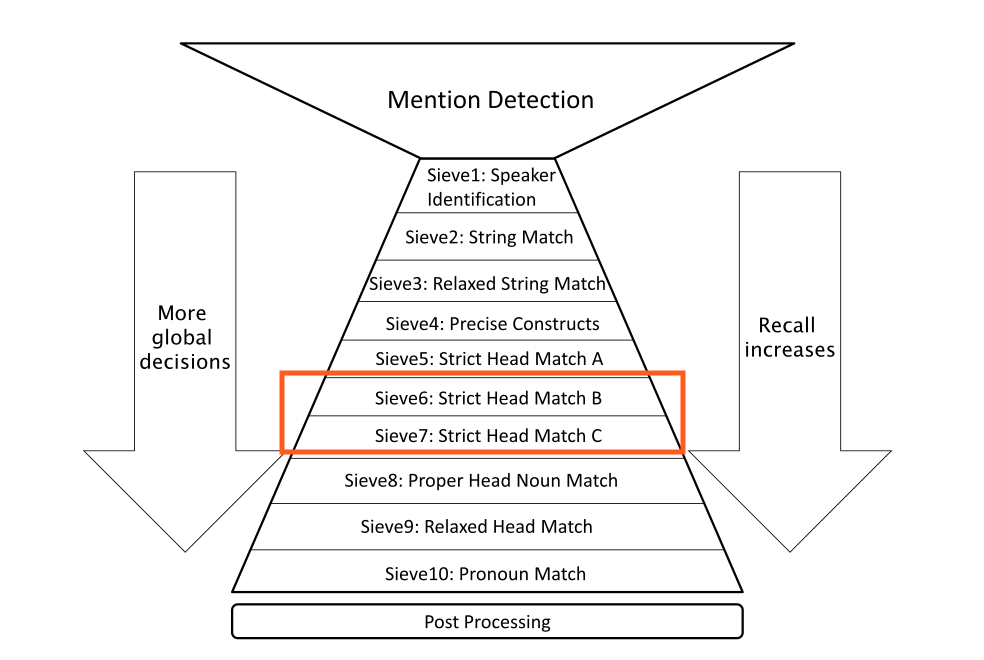
\includegraphics[scale=0.15]{sieve67.png} 
\bigskip

[John]$^{1}_{1}$ is [a musician]$^{1}_{2}$. [He]$^{3}_{3}$ played [a new song]$^{4}_{4}$.

[A girl]$^{5}_{5}$ was listening to [the song]$^{4}_{6}$.

“[It]$^{7}_{7}$ is [[my]$^{1}_{9}$ favorite]$^{7}_{8}$,” [John]$^{1}_{10}$ said to [her]$^{11}_{11}$.

\end{frame}

\begin{frame}{Proper Head Noun Match}

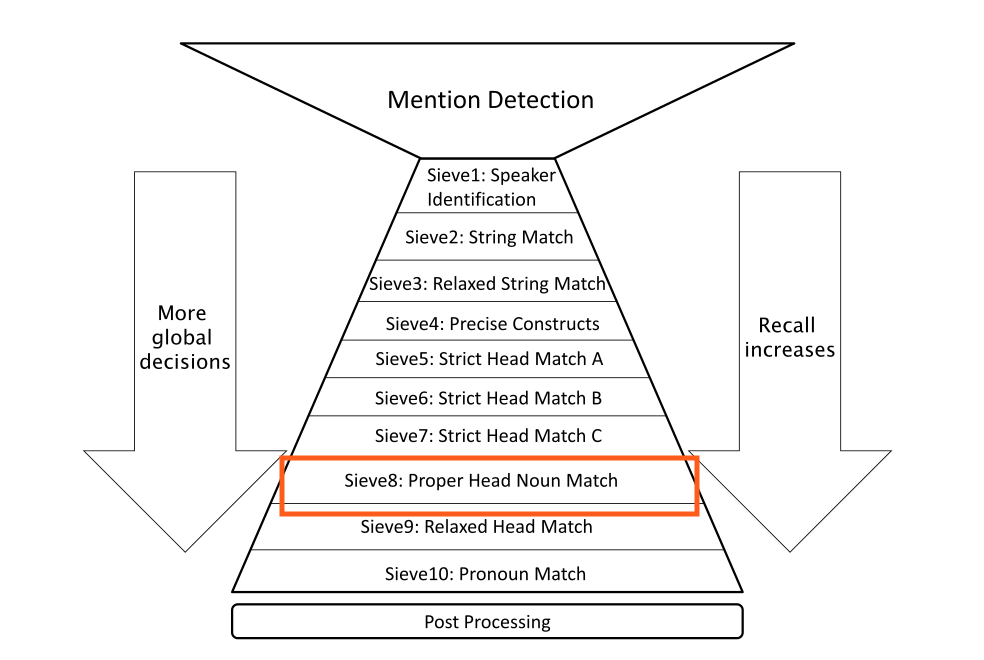
\includegraphics[scale=0.15]{sieve8.png} 
\bigskip

[John]$^{1}_{1}$ is [a musician]$^{1}_{2}$. [He]$^{3}_{3}$ played [a new song]$^{4}_{4}$.

[A girl]$^{5}_{5}$ was listening to [the song]$^{4}_{6}$.

“[It]$^{7}_{7}$ is [[my]$^{1}_{9}$ favorite]$^{7}_{8}$,” [John]$^{1}_{10}$ said to [her]$^{11}_{11}$.

\end{frame}

\begin{frame}{Relaxed Head Match}

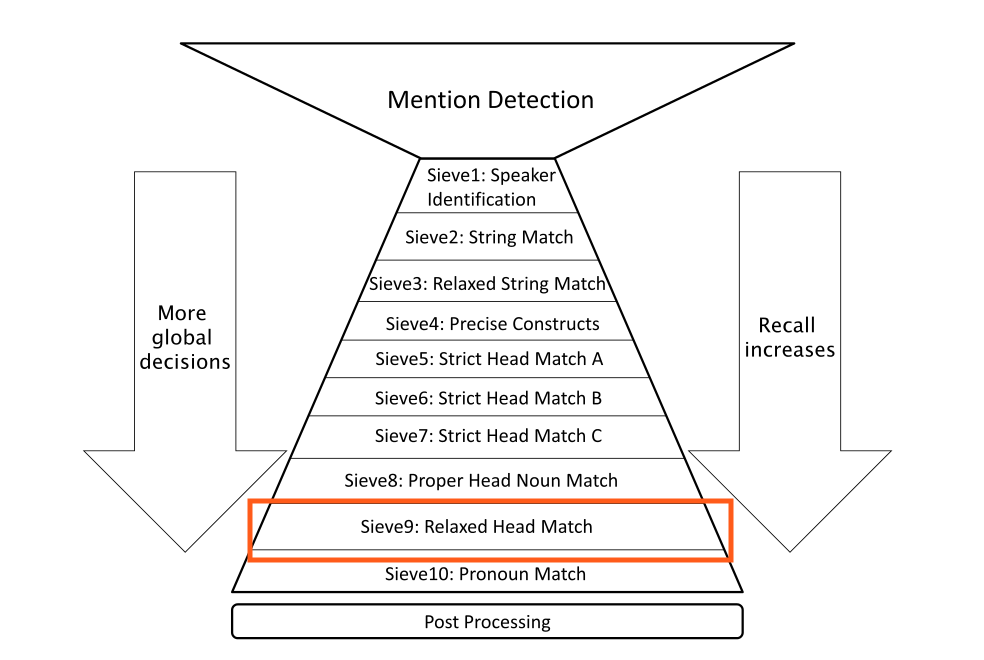
\includegraphics[scale=0.15]{sieve9.png} 
\bigskip

[John]$^{1}_{1}$ is [a musician]$^{1}_{2}$. [He]$^{3}_{3}$ played [a new song]$^{4}_{4}$.

[A girl]$^{5}_{5}$ was listening to [the song]$^{4}_{6}$.

“[It]$^{7}_{7}$ is [[my]$^{1}_{9}$ favorite]$^{7}_{8}$,” [John]$^{1}_{10}$ said to [her]$^{11}_{11}$.

\end{frame}

\begin{frame}{Pronoun Match}

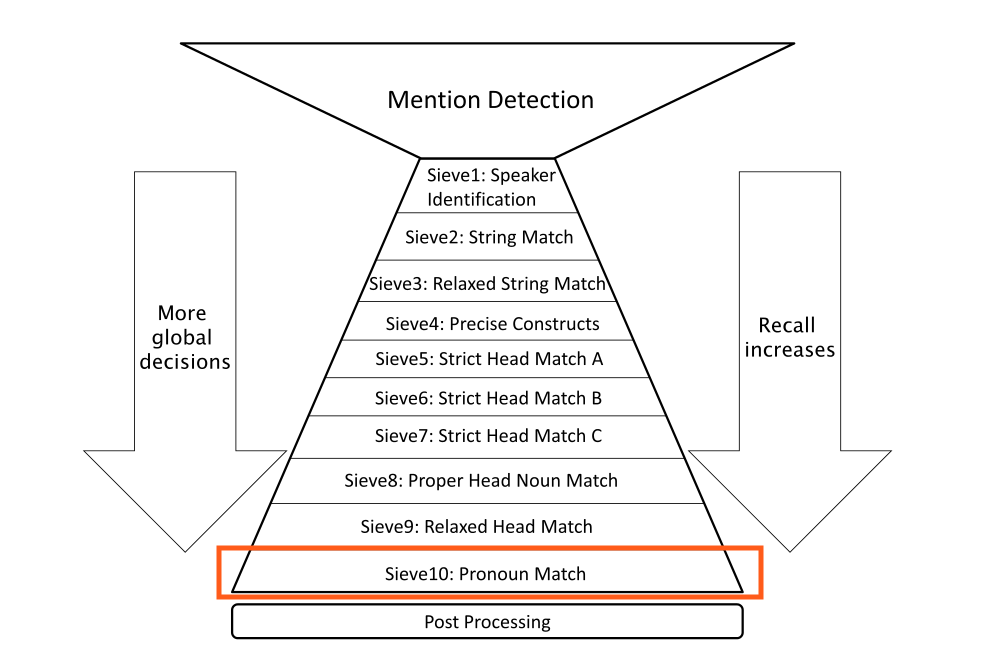
\includegraphics[scale=0.15]{sieve10.png} 
\bigskip

\textbf{[John]}$^{1}_{1}$ is [a musician]$^{1}_{2}$. \textbf{[He]}$^{1}_{3}$ played [a new song]$^{4}_{4}$.

\textbf{[A girl]}$^{5}_{5}$ was listening to \textbf{[the song]}$^{4}_{6}$.

“\textbf{[It]}$^{4}_{7}$ is [[my]$^{1}_{9}$ favorite]$^{4}_{8}$,” [John]$^{1}_{10}$ said to \textbf{[her]}$^{5}_{11}$.

\end{frame}

\begin{frame}{Post Processing + Final Output}

[John]$^{1}_{1}$ is \textbf{a musician}. [He]$^{1}_{3}$ played [a new song]$^{4}_{4}$.

[A girl]$^{5}_{5}$ was listening to [the song]$^{4}_{6}$.

“[It]$^{4}_{7}$ is \textbf{[my]$^{1}_{9}$ favorite},” [John]$^{1}_{10}$ said to [her]$^{5}_{11}$.


\begin{quote}
\bigskip
\normalfont{\large{
[John]$^{1}_{1}$ is a musician. [He]$^{1}_{3}$ played [a new song]$^{4}_{4}$.

[A girl]$^{5}_{5}$ was listening to [the song]$^{4}_{6}$.

“[It]$^{4}_{7}$ is [my]$^{1}_{9}$ favorite,” [John]$^{1}_{10}$ said to [her]$^{5}_{11}$.}}
\end{quote}
\end{frame}

\begin{frame}{References}
\nocite{*}
\bibliographystyle{abbrv}
\bibliography{lit}
\end{frame}

\end{document}